\section{Experiments}
\label{sec:experiments}
\begin{figure}
\centering
\subfloat[The sensor node]{\label{fig:carParkSensor1}\figurehalfwidth{carParkSensor1.JPG}}
\subfloat[The light sensor]{\label{fig:carParkSensor2}\figurehalfwidth{carParkSensor2.JPG}}
\qquad
\subfloat[Car park sensor deployment]{\label{fig:carParkDeployment}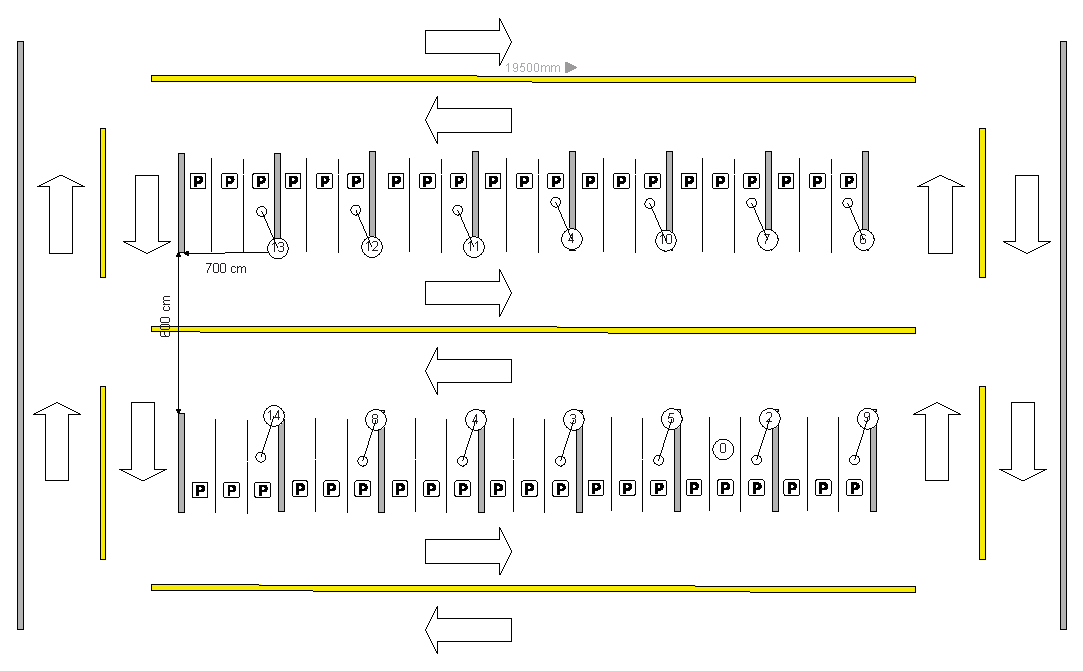
\includegraphics[width=.8\textwidth]{carParkDeployment}}
\caption{Car park experiment setup}
\label{fig:carParkSensor}
\end{figure}

In this section, based on our PSWare implementation, we use it to evaluate the performance of different event detection algorithms in different applications. In particular, we implemented and tested two event detection algorithms. The first one is TED \cite{lai:ted}, a distributed type-based event detection algorithm. TED uses optimization methods and select a subset of nodes from the network as event detectors. The second algorithm is opportunistic event detection mechanism where all the events are simply transmitted to the sink for detection with CTP \cite{ctp} provided by TinyOS. Events may be also detected opportunistically on their transmission paths. We compare the performance using the following metrics:
\begin{itemize}
\item Message cost: this is obtained by setting up a counter inside the sensor node. The counter will be written into flash after the experiment so that we can retrieve it.
\item Event detection delay: we measure the time between the subscription is disseminated and the event is notified.
\end{itemize}


\subsection{Application Case One: Car Park}
\begin{figure}
\centering
\subfloat[Message cost]{\label{fig:carParkResult1}\figurehalfwidth{carParkResult1}}
\subfloat[Delay]{\label{fig:carParkResult2}\figurehalfwidth{carParkResult2}}
\caption{Car park experiment results}
\label{fig:carParkResults}
\end{figure}
Our first application case is an intelligent car park \cite{tang:carpark}. We deployed some micaz sensor nodes for the application. For simplicity, we use light sensor to detect the presence of a vehicle. For better communication, the sensor nodes are attached close to the ceiling instead of on the ground. The light sensor on each node is connected through an extended cable as shown in Figure \ref{fig:carParkSensor}. 

The deployment of the sensor nodes is shown in Figure \ref{fig:carParkDeployment}. In such a system, the management is interested in the number of park spaces and the location of them \cite{tang:carpark}. The primitive events for such a system will be the availability of individual car park spaces. Based on the primitive event, if we want to get notified when the parking spaces near the exit become available, then we just need to define composite events which locate the spaces with certain IDs. Th event definitions are shown in Listing \ref{prog:carPark}. Here, the composite event takes two primitive events for parking space \(1\) and \(2\) which are close to the exit. The experimental results are shown in Figure \ref{fig:carParkResults}. In this application, we primarily consider only the message costs because the delay isn't that important in such a system. The message cost is highest during rush hour when there are a lot of cars entering and leaving the car park. For all the experiments as we can see, the message cost of TED is lower than that of opportunistic approach.

\begin{lstlisting}[caption=Event definition for a car park, label=prog:carPark]
Event ParkSpaceEvent {
	int id=System.id;
	int time=System.time;
	int light=System.light;
} where {
	light>THRESHOLD
}
Event CarParkEvent {
	int id=System.id;
} on {
	ParkSpaceEvent e1, e2;
} where {
	e1.id==1 ||
	e2.id==2 ||
	e1.time-e2.time<10
}
\end{lstlisting}

\subsection{Application Case Two: Transportation Systems}
Apart from intelligent car park, another related application is WSN-based vehicle detection and tracking \cite{lai:its}. The deployment is shown in Figure \ref{fig:itsSensor}.

\begin{figure}
\centering
\subfloat[Road side sensor nodes]{\label{fig:itsSensor1}\figurehalfwidth{itsSensor1.JPG}}
\subfloat[Sensor nodes on the lamp]{\label{fig:itsSensor2}\figurehalfwidth{itsSensor2.JPG}}
\caption{Sensor nodes for transportation systems}
\label{fig:itsSensor}
\end{figure}

The event definitions are shown in Listing \ref{prog:carEvent}.
\begin{lstlisting}[caption=Event definition for tracking vehicles, label=prog:carEvent]
Event CarEvent {
	int time=System.time;
	int magnetic=System.magnetic;
	int location=System.location;
} where {
	magnetic>THRESHOLD
}
Event SpeedEvent {
	int speed=(e1.location-e2.location)/(e1.time-e2.time);
} on {
	CarEvent e1, e2;
} where {
	e1.time>e2.time &&
	speed>THRESHOLD
}
\end{lstlisting}

Different from the car park application, such applications are more delay sensitive. The results are shown in Figure \ref{fig:itsResults}. Similar to the car park application, TED saves more energy than opportunistic approach while introducing a small amount of delay.
 
\begin{figure}
\centering
\subfloat[Message cost]{\label{fig:itsResult1}\figurehalfwidth{itsResult1}}
\subfloat[Delay]{\label{fig:itsResult2}\figurehalfwidth{itsResult2}}
\caption{Experiments on the roads}
\label{fig:itsResults}
\end{figure}

\subsection{Application Case Three: Indoor Monitoring}
Our final application is related to smart building. We consider the application scenario where the sensor nodes are deployed in a building so that the temperature can be monitored. Such an application can probably be useful for certain types of context aware pervasive applications. For example, the air conditioner can be adjusted if several adjacent rooms' temperature rises too fast. The primitive and composite event definitions are shown in Listing \ref{prog:indoorEvents}.

\begin{lstlisting}[caption=Event definition for indoor monitoring, label=prog:indoorEvents]
Event SingleTemp {
	int id=System.id;
	int temperature=System.temperature;
} where {
	temperature>THRESHOLD
}
Event CompositeTemp {
} on {
	SingleTemp e1, e2, e3;
} where {
	e1.id==1 &&
	e2.id==2 &&
	e3.id==4
}
\end{lstlisting}

The primitive event simply tests if the temperature passes certain threshold and the composite event is the conjunction of several primitive events. We deployed the some Micaz nodes in different rooms in our building as shown in Figure \ref{fig:indoorDeployment}.

\begin{figure}
\centering
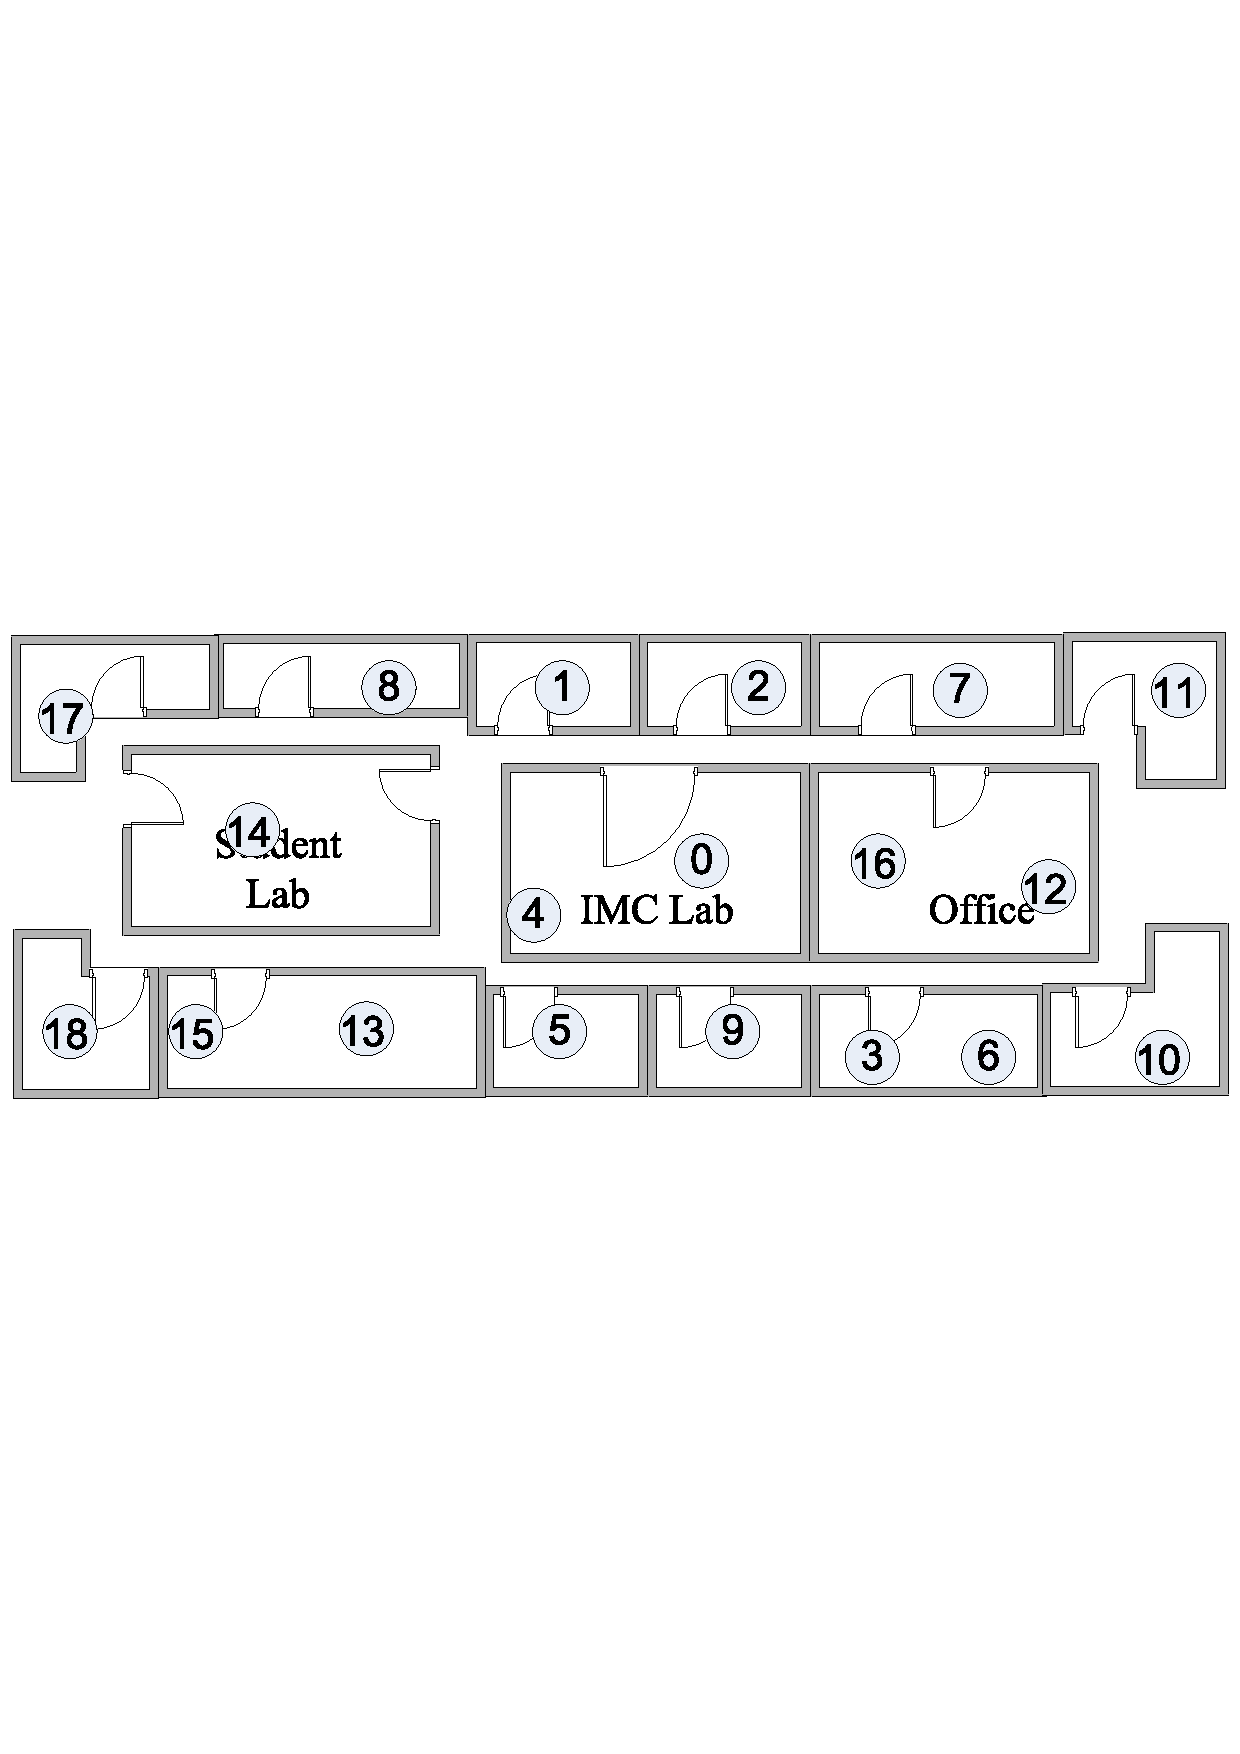
\includegraphics[width=.8\textwidth]{indoorDeployment}
\caption{Deployment of the senosr nodes for indoor monitoring}
\label{fig:indoorDeployment}
\end{figure}

The experimental results is shown in Figure \ref{fig:itsResults}. It is shown that TED can save the message cost by 10-20\%.

\begin{figure}
\centering
\subfloat[Message cost]{\label{fig:indoorResult1}\figurehalfwidth{indoorResult1}}
\subfloat[Delay]{\label{fig:indoorResult2}\figurehalfwidth{indoorResult2}}
\caption{Experiments for temperature monitoring}
\label{fig:indoorResult}
\end{figure}